\chapter{Databasen}

\section{Opbygning af databasen}

Logikken  bag databasen er at holde styr på reservationer, kunder, hoteller, værelser og faciliteter. 
Databasen er designet til at kunne håndtere reservationer af værelser på hoteller, 
og at kunne holde styr på kundernes informationer og hvilke faciliteter hotellerne tilbyder.

Dette medfører at databasen består af følgende tabeller:
\begin{itemize}
    \item Hotels
    \item Customers
    \item Rooms
    \item Reservations
    \item Facilities
    \item HotelFacilities
\end{itemize}

\subsection{Relationer og Multiplicity}

\begin{itemize}
    \item Et Hotel kan have mange Rooms (1 to Many)
    \item En Customer kan have mange Reservations (1 to Many)
    \item Et Room kan være del af en Reservation af gangen (1 to Many)
    \item Facilities er delt mellem Hotels gennem HotelFacilities (Many to Many)
\end{itemize}

\subsection{3NF tilstand}
Alle tabeller er i 3NF fordi:
\begin{enumerate}
    \item De er i 1NF da alle attributter er \emph{atomiske} - ingen grupper gentages eller indeholder mere end én værdi.
            Dette ses bl.a. ved at HotelFacilities er en relationstabel mellem Hotel og Facility.
    \item De er i 2NF da der ikker er noget \emph{partiel afhængighed} - Non-key kolonner afhænger udelukkende af PK. 
            Dette ses bl.a. ved at Hotel har en relation til Facaility, istedet for at indeholde Facility som attribut.
    \item Der er ingen \emph{transitiv afhængighed} - Non-key kolonner afhænger kun af PK.
            Dette ses bl.a. ved at Room har en relation til Hotel, istedet for at indeholde Hotel som attribut.
\end{enumerate}

\section*{Diagrammer}
Diagrammerne burde være så simple, at de er selvforklarende. DMD er lavet først og ud fra Many-to-many forholdet mellem hoteller og faciliteter, giver det anledning til et indextable (HotelFacilities).
HotelFacilities anskues ikke i DMD som værende en selvstædig entity men mere måde at styre relationen mellem Hotel og Facilities.

\begin{figure}
    \centering
    \begin{subfigure}[b]{0.45\textwidth}
        \centering
        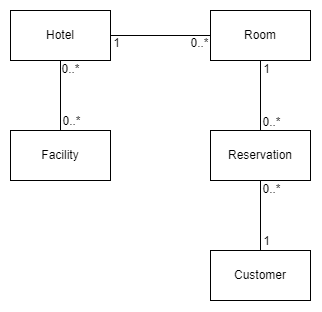
\includegraphics[width=\textwidth]{figures/SWD_Domain_HotelManagement.png}
        \caption{Domain Model Diagram}\label{DomainModelDiagram}
    \end{subfigure}
    \hfill
    \begin{subfigure}[b]{0.45\textwidth}
        \centering
        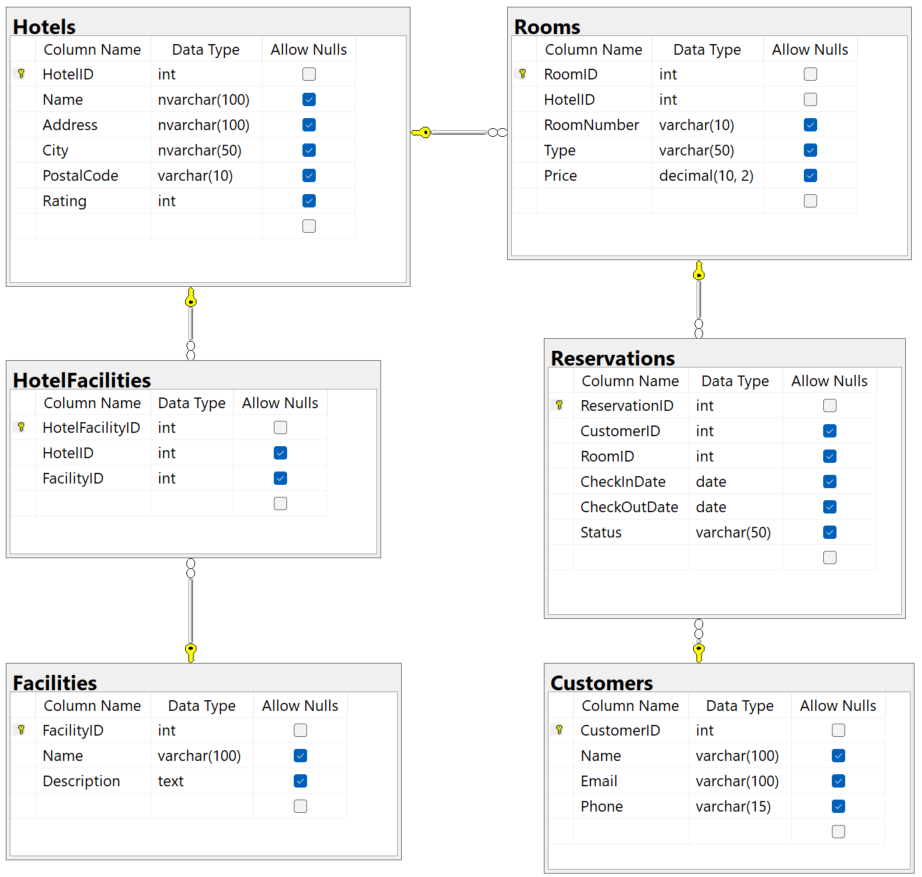
\includegraphics[width=\textwidth]{figures/SWD_ERD_HotelManagement.png}
        \caption{Entity Relationship Diagram}\label{EntityRelationDiagram}
    \end{subfigure}
    \caption{Domain Model and Entity Relationship Diagrams}
\end{figure}

\subsection{Domain Model Diagram}
Se figur 1. Dette DMD er der udelukkende entities, muliplicitet og relationer.
Dette giver input til hvordan DB skal designes udfra de enkelte tabeller og deres relationer til hinanden.

\subsection{Entity-Relationship Diagram}
Se figur 1. ERD er genereret ud fra tabellerne i databasen, og viser relationerne mellem tabellerne, deres PK, FK og datatype.